% !TeX spellcheck = en_US
\section{Problem 3}

LVQ (Learning Vector Quantization) is a type of artificial neural network algorithm used for supervised learning. It belongs to the category of competitive learning algorithms and is particularly effective for classification tasks.

\begin{figure}[htpb]
	\centering
	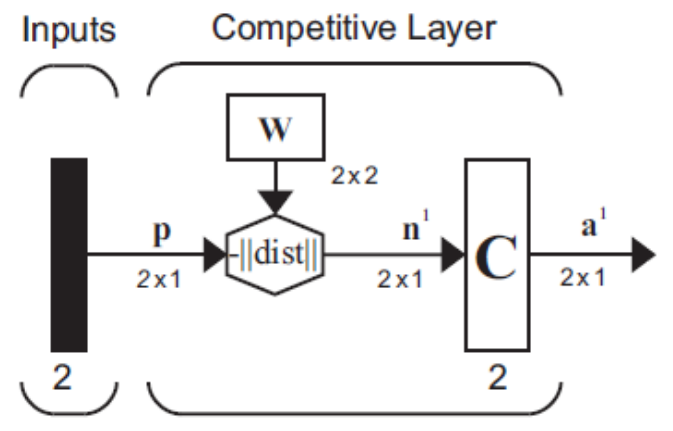
\includegraphics[width=0.4\linewidth]{../Problem 3/prob3_lvq_nn.png}
	\caption{Given neural network.}
\end{figure}

The following $-||w_i - p||$ applies to every $n^1_i$. Also, we can also state that $a^1 = compet\left(n^1\right)$, where $compet$ is competitive learning layer.

During training, the distance between $a$ and $w$ is calculated using $dist = norm\left(p-w_{1,2}\right)$ and judging by whose norm is greater, the winning neutron gets updated.
Also, the presentation order of the vectors during training is: $p_1, p_2, p_3, p_2, p_3, p_1$.

All initial values are presented below:
\[
p_1 = \left[
\begin{array}{c}
	1\\1
\end{array}
\right], \quad
p_2 = \left[
\begin{array}{c}
	-1\\2
\end{array}
\right], \quad
p_3 = \left[
\begin{array}{c}
	-2\\-2
\end{array}
\right], \quad
w_1 = \left[
\begin{array}{c}
	0\\1
\end{array}
\right], \quad
w_2 = \left[
\begin{array}{c}
	1\\0
\end{array}
\right]
\]

In order to reduce unnecessary computations, we implemented a convergence control that stops training when weights have very small differences with each other.\\

After letting the network converge, we have as final weights the following:
\begin{center}
	\textit{\small Training converged at epoch 10.}
\end{center}
\[
w_1 = \left[
\begin{array}{c}
	-2\\-2
\end{array}
\right], \quad
w_2 = \left[
\begin{array}{c}
	0.2\\1.4
\end{array}
\right]
\] 

Finally, in figure~\ref{fig:prob3_weights_over_epoch} we can see the weights over epochs during training.
The code for this is in file \verb|prob3.py|.

\begin{figure}[htpb]
	\centering
	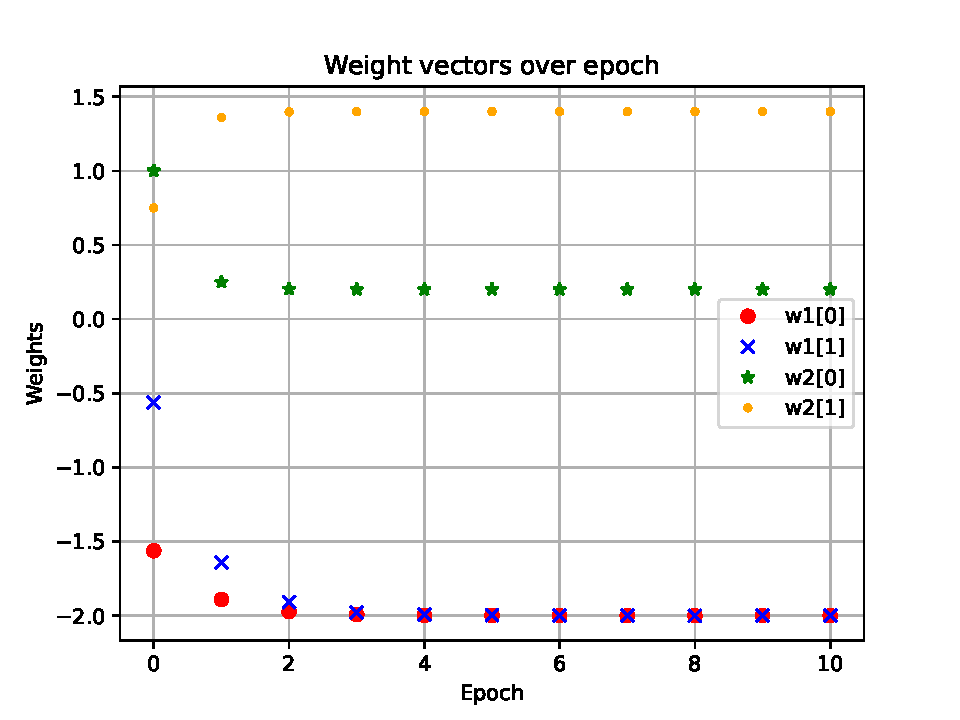
\includegraphics[width=0.47\linewidth]{../Problem 3/prob3_weights_over_epoch.pdf}
	\caption{Weights over epoch during training.}
	\label{fig:prob3_weights_over_epoch}
\end{figure}
\vspace{3mm}
